\chapter{Technische uitvoering}
In wat volgt, worden alle componenten (zowel hardware als software) uitvoerig besproken en wordt een verantwoording gegeven van de ontwerpkeuzes.
Dit hoofdstuk wordt opgedeeld in drie onderdelen: sectie \ref{sec:localization} lokalisatie, sectie \ref{sec:drone_control} drone aansturing en sectie \ref{sec:visualization} visualisatie.\\

Figuur \ref{fig:setup} toont de hardware setup, aangevuld met de gebruikte protocollen.\\
\begin{figure}[p]
	\centering
	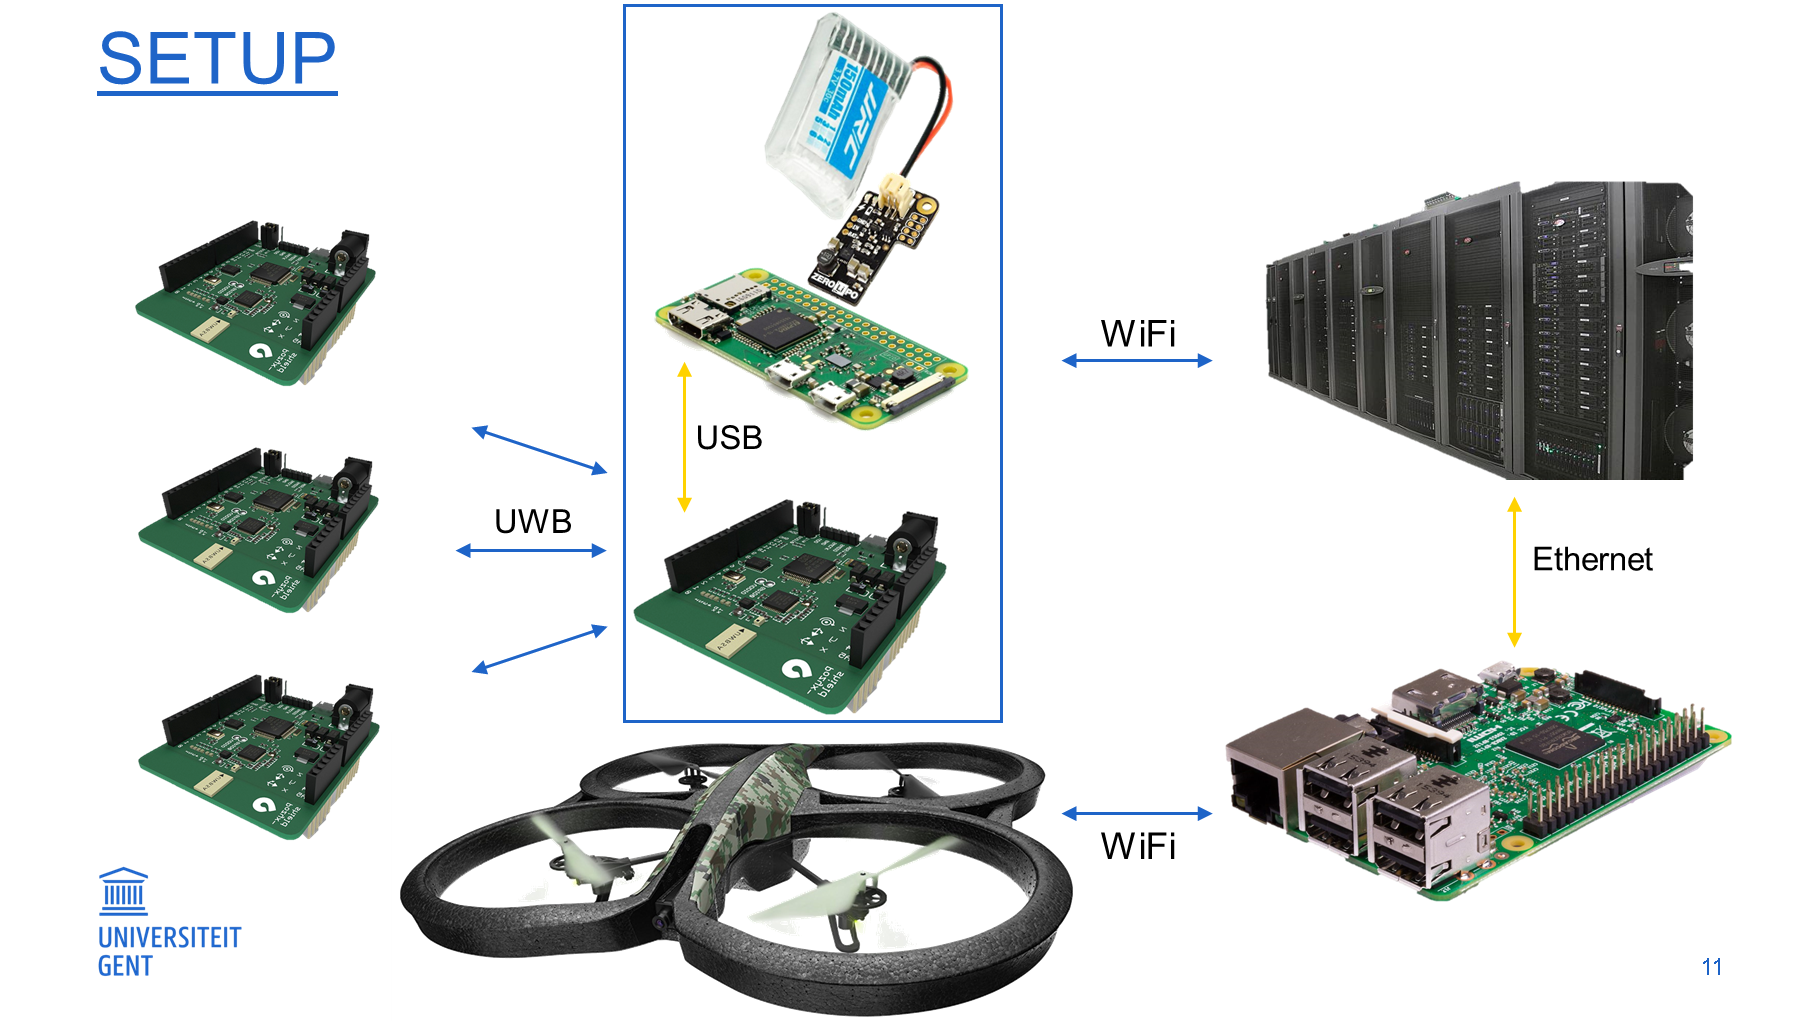
\includegraphics[width=\textwidth]{Setup}
	\caption[Setup]{Hardware setup, aangevuld met protocollen.}
	\label{fig:setup}
\end{figure}

De eerste beslissing omtrent hardware was het uitzoeken van de drone.
Hier werd geopteerd voor de Parrot\footnote{\url{https://parrot.com}} AR.Drone 2.0 Elite Edition met jungle camo.
De belangrijkste argumenten voor deze keuze zijn de kostprijs (\SI{116.71}{\euro{}}), de vluchtduur (\SI{12}{\min}) en het laadvermogen.
De meeste types drone die een lading van zo'n \SI{100}{\g} kunnen dragen, kosten minstens \SI{250}{\euro{}}.
Dit type is echter al even niet meer in productie, waardoor de prijs enorm gezakt is.
Een goedkopere drone met hetzelfde draagvermogen kon niet gevonden worden.\\

Ook voor het software gedeelte is deze drone een goede keuze. Parrot stelt een SDK, die toelaat om de drone via wifi aan te sturen en vlucht gegevens op te halen, openbaar ter beschikking.
Er bestaan reeds bibliotheken, waarvan er in dit project ook gebruik gemaakt wordt.\\

De frontale camera op de drone zou kunnen dienen om barcodes in te scannen, maar dat onderdeel werd niet onder de doelstellingen van dit project gedefiniëerd.
De drone bezit ook nog een ultrasone sensor om de hoogte ten opzichte van de vloer te meten en een naar de grond gerichte camera die toelaat dat de drone stabiel kan blijven zweven boven dezelfde positie.\\

Een tweede beslissing gaat over het opsplitsen van de on- en off-board controller.
Oorsponkelijk was de bedoeling om slechts één controller op de drone te plaatsen, die instaat voor communicatie met de Mosquitto server en aansturing van de drone.
Dit ontwerp brengt een groot probleem met zicht mee: de Raspberry Pi\footnote{\url{https://raspberrypi.org}} Zero W moet verbonden zijn met twee netwerken.\\
Een mogelijke manier om dit te bereiken is om een wifi dongle in de USB interface te pluggen, maar deze was reeds in gebruik genomen door de Pozyx\footnote{\url{https://www.pozyx.io}} tag.
Het is ook mogelijk om met de Pozyx tag verbinden via een seriële poort en zo de USB interface vrij te houden, maar dan stijgt het gewicht van de controller noemenswaardig door de extra kabels, adapter en wifi dongle.\\
Een andere piste die onderzocht werd, was om een wifi chip te verbinden met een seriële poort van de Raspberry Pi.
Er werd geöpteerd voor de Adafruit\footnote{\url{https://adafruit.com}} HUZZAH.
Dit is een \textit{breakout} van de ESP8266 wifi chip.
Opnieuw brengt dit enig gewicht met zich mee, maar vooral het stroomverbruik is nu een probleem.
Ook functioneert deze chip niet als een gewone wifi interface, maar moet hij aangesproken worden via commando's op de seriële poort.
Dit zorgt er voor dat de Node.js library onbruikbaar wordt.\\
De gekozen oplossing om dit probleem te omzeilen is de volgende: een extra off-board controller dat het aansturen van de drone voor z'n rekening zal nemen.
Meer over de off-board controller is te vinden in sectie \ref{sec:offboard_controller}.

\section{Lokalisatie} \label{sec:localization}
In theorie is het mogelijk om, als een drone op een gekende locatie (met een gekende oriëntatie) vertrekt, deze zonder enige input informatie of correcties een reeks vluchtbewegingen door te geven zodat een voorgeprogrammeerde route gevolgd wordt.
In de praktijk wordt dit echter bemoeilijkt door ongekende externe factoren. Denk bijvoorbeeld aan een ongekend obstakel dat plots het pad van de drone kruist of een ventilatieschacht die de drone uit positie blaast.
Ook het opstijgen gebeurt niet vlekkeloos, waardoor hij met een foutieve oriëntatie aan zijn tocht zou beginnen.
Daarom is het nodig dat de specifieke locatie van het toestel in de ruimte op elk ogenblik gekend is.\\

Als de drone tussen twee rekken met een doorgang van \SI{1}{\m} moet kunnen vliegen, dan moet de nauwkeurigheid van lokalisatie in de grootteorde van \SI{0.1}{\m} liggen.
Veelgebruikte lokalisatie-technologieën zoals gps, wifi en bluetooth zijn te onnauwkeurig voor deze toepassing.
Ultra-wideband (UWB) komt deze noden tegemoet.
Dit is een vrij recente techniek met een nauwkeurigheid in de grootteorde van \SI{0.1}{\m}, wat volstaat om de drone indoor te kunnen lokaliseren.
De locatiebepaling gebeurt aan de hand van een controller op de drone, die bestaat uit een UWB component, een Raspberry Pi Zero W en een Lithium-ion Polymeer (LiPo) batterij.\\

\subsection{Ultra-wideband} \label{sec:uwb}
Er werden twee verschillende opties vergeleken (cf. tabel \ref{tab:decavspozyx}) die als mogelijke ultra-wideband (UWB) component zouden kunnen dienen: de DecaWave DWM1001 en een Pozyx tag.
De DecaWave DWM1001 is een goedkope, lichte en compacte module. Lokalisatie werkt bij deze chip echter niet out-of-the-box, en het implementeren van de lokalisatie zou geen makkelijke programmeertaak zijn, mede doordat de communicatie met de chip niet evident is.
Ook was deze module niet direct beschikbaar.
Daarom werd er gekozen om beroep te doen op de Pozyx-hardware, ontwikkeld door een spin-off van de UGent.
Deze zijn duurder, zwaarder en groter, maar waren direct beschikbaar.
De begeleiders hadden hier ook al ervaring mee.
Voor de gebruikte drone is het minieme gewichtsverschil van de Pozyx tag niet echt een probleem.
Er moet echter wel in het achterhoofd houden worden dat meer massa de stabiliteit en vliegminuten in negatieve zin beïnvloedt.\\

Op gekende locaties in de ruimte worden Pozyx ankers opgehangen.
De mobiele tag, die onderdeel uit maakt van de controller, kan om de beurt de verschillende ankers aanspreken, en opvragen hoe ver hij van hen verwijderd is.
Deze data wordt dan verwerkt door een Raspberry Pi Zero W.
\begin{table}[p]
	\centering
	\begin{tabular}{ | l | c | c | } \hline
		& DecaWave DWM1001 & Pozyx \\
		\hline 
		\hline
		Prijs (\euro{}) & 20 & 135 \\ 
		\hline
		Massa (g) & 4 & 12 \\ 
		\hline
		Afmetingen ($mm \times mm$) & $19.1 \times 26.2$ & $60 \times 53$ \\ 
		\hline
	\end{tabular}
	\caption[Vergelijking DecaWave DWM1001 en Pozyx tag]{Vergelijking DecaWave DWM1001 en Pozyx tag.}
	\label{tab:decavspozyx}
\end{table}

\subsection{Raspberry Pi Zero W} \label{sec:zerow}
Het aansturen van de Pozyx tag gebeurt met een Raspberry Pi Zero W.
De verbinding tussen de Pozyx tag en de Raspberry Pi wordt gelegd via een USB On-The-Go (OTG) kabel, waarvan beide uiteinden van het type micro-USB zijn.
Deze kleine, lichte computer (slechts \SI{9}{\g}) zorgt voor de verwerking van de data die de tag genereert.
Hij is verbonden met het internet en kan zo communiceren met een Mosquitto server die gebruikt wordt voor de verwerking en distributie van de data.
Communicatie met de Mosquitto server werkt via het MQTT-protocol.
Twee belangrijke concepten zijn het \textit{publishen} en het \textit{subscriben} op een bepaalde topic op de server.
Aan de kant van de on-board controller wordt er vooral data verstuurd naar de server (\textit{publish}), terwijl de onderdelen die nog volgen vooral data uitlezen (\textit{subscribe}).\\

De Raspberry Pi stuurt de Eulerhoeken, voor de oriëntatie van de drone, en de afstanden tot de verschillende ankers naar de server.
Door middel van een \textit{particle filter} die reeds beschikbaar was worden deze afstanden omgezet naar een precieze locatie. De visualisatie-software en de software voor het aansturen van de drone luisteren naar deze topics en kunnen deze data verder gebruiken.
Tijdens de start van dit project leverde deze filter de locatie in 2D (intussen ook in 3D), daarom wordt er hier gebruik gemaakt van de ultrasone sensor van de drone voor het bepalen van de hoogte.\\

Naarmate de drone in een groter magazijn rondvliegt, hangen er ook meer ankers.
Een belangrijk aspect naast nauwkeurigheid, is de snelheid waarmee hij zijn locatie kan updaten.
Wanneer de drone zich verplaatst kan het zijn dat hij buiten het bereik is van sommige ankers.
Alle ankers aanspreken zou er dan voor kunnen zorgen dat de update tijd vertraagd.
Een mogelijke manier om dit te verhinderen zou zijn dat de drone enkel de vier ankers aanspreekt die het dichts bij hem in de buurt liggen.

\subsection{Power supply} \label{sec:power_supply}
Een Lithium-ion Polymeer (LiPo) batterij moet de controller gedurende ongeveer een kwartier van stroom kunnen voorzien, aangezien de drone ook ongeveer \SI{15}{\min} lang in de lucht kan blijven.
De controller met de aanwezige Pozyx tag heeft gedurende een kwartier ongeveer \SI{350}{\mA} nodig.
Er werd gekozen voor een batterij van \SI{500}{\mA\hour} om pieken op te kunnen vangen.
Deze batterij kan gedurende een kwartier zo'n \SI{2000}{\mA} leveren aan de controller.\\

Er wordt een LiPo SHIM tussen de Raspberry Pi Zero W en de LiPo batterij geplaatst, omdat de Rasberry Pi op \SI{5}{\V} opereert i.p.v. \SI{3.7}{\V}.
Deze zal niet enkel het voltage omvormen, maar bezit ook een indicator die inschakelt wanneer de batterij bijna leeg is.

\section{Drone aansturing} \label{sec:drone_control}
\subsection{Off-board controller} \label{sec:offboard_controller}
Er wordt gebruik gemaakt van een Raspberry Pi 3 B om de drone effectief aan te sturen.
Deze heeft de mogelijkheid om met twee netwerken tegelijk te verbinden.
De ethernet interface wordt gebruikt om verbinding te maken met het internet (meer bepaald de Mosquitto server), terwijl de wifi interface gebruikt wordt om met het netwerk van de drone te verbinden.\\

Het eerste waarover een beslissing moest genomen worden was het al dan niet gebruiken van een reeds bestaande library, en zo ja de welke?
Bij de keuze van drone werd beschikbaarheid van documentatie steeds in het achterhoofd gehouden waardoor er veel opties beschikbaar waren. Volgende opties werden onderzocht:
\begin{itemize}
\item python-ardrone
\item YADrone
\item AR Drone Simulink Development-Kit
\item AR Drone Toolkit for LabVIEW
\item Nodecopter
\end{itemize}

De finale keuze werd gemaakt tussen python-ardrone en Nodecopter. Doorslaggevend voor de keuze voor Nodecopter was de zeer grote beschikbaarheid van documentatie en extra modules.\\

Aangezien er via Python werd gecommuniceerd zorgde dit er wel voor dat de drone aansturing moest worden opgesplitst in twee delen. Enerzijds het Node.js deel dat de commando's doorstuurt naar de drone, en anderzijds het python script dat de positie en \textit{waypoints} ophaalt van de Mosquitto server en omvormt tot instructies voor de drone.

\subsection{Communiceren met de drone via Nodecopter}
Aangezien alle berekeningen reeds worden gedaan in het Python script is de Node.js kant niet veel meer dan een tussenstuk dat alle data ontvangt op een lokale socket en meteen doorstuurt naar de drone door middel van Nodecopter commands.
De enige andere noemenswaardige feature is dat het script ook de hoogte ontvangt van de drone en dit terugstuurt over dezelfde socket.
Dit gebeurt in parallel met de besturingslus zodanig dat deze niet moet wachten op de hoogte.\\

Er wordt gebruik gemaakt van de 'node-ar-drone' bibliotheek van Nodecopter.
Dit is de standaard library voor het besturen van de drone. Deze laat toe om de drone high level aan de sturen.
Er kan simpelweg een drone object worden aangemaakt waarop functies als 'forward' of 'left' kunnen opgeroepen worden met als argumenten een fractionele snelheid tussen 0 (stil) en 1 (maximum snelheid).\\

Het gebruik van de 'ardrone-autonomy' library werd ook onderzocht. Dit is een uitbreiding op de standaard library die toelaat om de drone nog meer high-level aan te sturen aan de hand van afstand en draaihoek in plaats van snelheid.
Al snel werd echter duidelijk dat deze library niet accuraat genoeg is  voor indoor vluchten met kleine foutmarges.
Een flowchart voor dit deel is te vinden in figuur \ref{fig:flowchart_server}.
\begin{figure}[p]
	\centering
	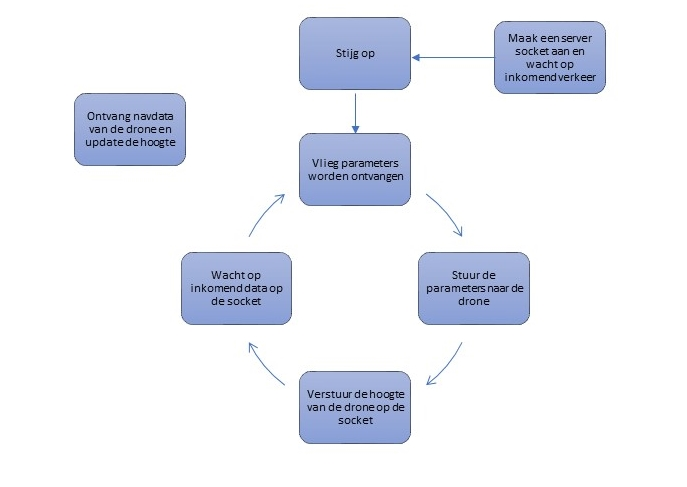
\includegraphics[width=\textwidth]{images/node_server_flowchart}
	\caption[Flowchart van de server]{Flowchart van de server. Merk op dat het ontvangen van navdata los staat van de lus aangezien dit parallel gebeurt.}
	\label{fig:flowchart_server}
\end{figure}

\subsection{Data verwerken in Python}
Het Python script levert het meeste werk.
De locatie verkregen van de Mosquitto server wordt gebruikt om te berekenen tegen welke snelheid en in welke richting de drone moet vliegen.
Deze informatie wordt dan doorgestuurd over een lokale socket naar het Node.js script op poort 8124.
Een flowchart voor dit deel is te vinden in figuur \ref{fig:flowchart_client}.
\begin{figure}[p]
	\centering
	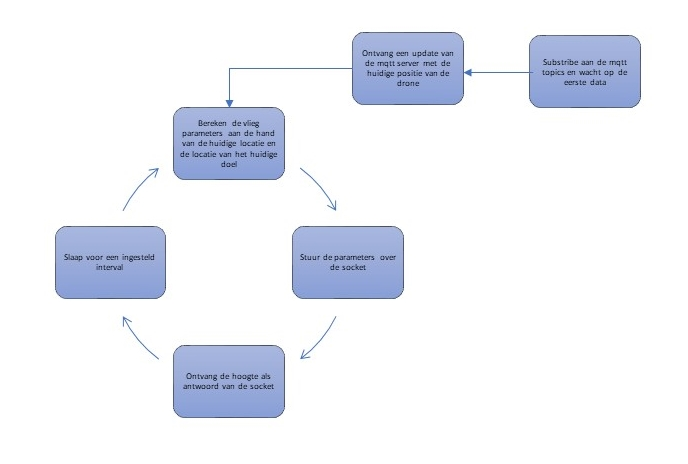
\includegraphics[width=\textwidth]{images/python_client_flowchart}
	\caption[Flowchart van de client]{Flowchart van de client.}
	\label{fig:flowchart_client}
\end{figure}

\subsubsection{Vliegalgoritme 1}
Een eerste poging bestond eruit de informatie omtrent de locatie te gebruiken en om te zetten in twee snelheden, namelijk een voorwaartste snelheid en een hoeksnelheid.
Het idee was simpel: de drone draait zich telkens in de juist richting en gaat dan vooruit met een snelheid linear afhankelijk met de afstand tot het doel.
Indien hij binnen een bepaalde radius van het \textit{waypoint} is zal hij de coordinaten updaten en naar het volgende punt vliegen.
Hoewel dit idee theoretisch goed klinkt was dit praktisch moeilijker uit te voeren.
Het voornaamste probleem was dat het vooruit vliegen en draaien in parallel gebeurde, wat er voor zorgde dat de drone eerder in een boog vloog in plaats van rechtdoor.

\subsubsection{Vliegalgoritme 2}
In een tweede poging werd enkel gebruik gemaakt van de lineare richtingen van de drone, en niet geroteerd.
Het komt er op neer dat de drone enkel naar voor, achter, links of rechts gaat, en zijn \textit{heading} steeds in dezelfde richting wijst.
Dit bleek een accurater algoritme, dus werd hier mee verder gewerkt. Een grote beperking in de setup is dat de hoek berekend door middel van de Pozyx tags relatief is, en telkens anders is na het opstarten.
Dit heeft als gevolg dat de drone telkens gealligneerd met het assenstelsel moet opstijgen.
Ook hier neemt de snelheid linear af, tot de drone binnen een gegeven afstand van het punt is.
Dan zet hij de parameter ’done’ op true, en kan er over gegaan worden naar het volgende waypoint in de lijst.

\section{Visualisatie} \label{sec:visualization}
Er werd besloten om een component aan het project toe te voegen, dat instaat voor de routebepaling en -controle, om het geheel gemakkelijk bruikbaar te maken.
Hiervoor werden eerst en vooral bestaande mogelijkheden verkend.
Aangezien deze ontoereikend leken voor dit project werd besloten om dit onderdeel zelf uit te werken met behulp van Unity\footnote{\url{https://unity3d.com/}}.

\subsection{Bestaande visualisatiemogelijkheden} \label{sec:opties}
Er werden eerst bestaande opties verkend, om geen onnodig werk te verrichten.
De minimumvereisten waren dat zowel de huidige positie van de drone in de ruimte als de te volgen route in drie dimensies weergegeven moesten kunnen worden.
Daarnaast moest de route ook op een inituïtieve manier ingegeven kunnen worden.
Tot slot werd ook verwacht dat de route gecontroleerd werd op eventuele problemen onderweg, zoals collisies met obstakels.\\

Geen van alle bestaande opties leek echter aan de eisen te voldoen.
De optie die door de begeleiders aangereikt werd, voldeed aan de meeste vereisten.
Het enige probleem was dat de positie en route niet in 3D weergegeven konden worden.
Er werd al snel beslist dat dit een te grote tekortkoming was om er mee te werken.
De enige optie die over bleef was om zelf aan de slag te gaan en een applicatie te ontwikkelen die aan alle eisen voldeed.

\subsection{Applicatie} \label{sec:unity}
Het ontwikkelen van de applicatie gebeurde in verschillende fasen. In elke fase werd het bestaande ontwerp verder verfijnd en uitgebreid met nieuwe functionaliteiten om zo tot het eindresultaat te komen.\\

In de eerste fase was het de bedoeling om de ruimte en de drone te modelleren.
Het nabootsen van de ruimte bestond erin om via elementaire 3D-vormen een zo accuraat mogelijk model voor de gehele ruimte te creëren.
Elk obstakel moest daarbovenop van een \textit{collider} voorzien worden opdat er later op collisies met de drone gecheckt zou kunnen worden.
Deze \textit{colliders} zijn standaard componenten die Unity gebruikt om botsingen te detecteren en waren reeds voorhanden.
Voor de drone werd een gratis model\footnote{\url{https://clara.io/view/1c6e9fef-d10d-42d0-8493-d619c2b95f55}} rechtstreeks in Unity geïmporteerd.\\

Om de gemodelleerde ruimte aan te passen moet de scene in de Unity editor aangepast worden.
Voor de muren, vloer en obstakels zijn alleen maar standaardvormen gebruikt.
De \textit{colliders} worden hier automatisch aan toegevoegd.
Het volstaat dus om ofwel de bestaande objecten te verslepen en herschalen ofwel te verwijderen en nieuwe toe te voegen.
Hierbij moet wel in het achterhoofd gehouden worden dat de oorsprong van het Unity model gelijk moet liggen met de oorsprong volgens de server.
Om kleuren aan de obstakels toe te voegen kunnen de gemaakte \textit{materials} uit de map Assets/Colors simpelweg op de obstakels in de scene gesleept worden.\\

De tweede fase bestond erin om de drone live te kunnen volgen in het model van de ruimte.
Dit wordt met behulp van een zelfgeschreven C\# script gedaan.
Dit script is in staat om de locatie van de echte drone van de server te halen en met behulp van die informatie het model te updaten.
Hierdoor wordt de drone op de correcte plaats in het model weergegeven. De grootste uitdaging in deze fase was het verbinden met de server vanuit het script en de informatie op de correcte manier verwerkt te krijgen. Een probleem dat hier tevoorschijn kwam, was dat Unity een ander assenstelsel hanteert dan de server. Dit kon met een simpele coördinatentransformatie opgelost worden en werd voor de rest van het project in het achterhoofd gehouden.\\

Toen de drone live weergegeven kon worden, was de volgende uitdaging om routes naar de drone te kunnen verzenden.
Om input van de gebruiker mogelijk te maken werd een Graphical User Interface (GUI) gemaakt.
Het script genereert \textit{waypoints} op locaties die door de gebruiker in de aangewezen velden ingegeven werden.
Wanneer de gebruiker deze punten in de juiste volgorde ingegeven heeft worden deze met een druk op de knop op de server gezet, waar ze afgehaald kunnen worden om de drone aan te sturen.
De locaties worden in JavaScript Object Notation (JSON) doorgegeven, opdat verwerking ervan gemakkelijk zou kunnen gebeuren.
Problemen die in deze fase de kop opstaken waren het dynamisch genereren van elementen in het 3D model en het versturen van de locaties naar de server.
Het versturen naar de server bleek, dankzij de beschikbare voorbeeldcode, geen groot obstakel.
Voor het dynamisch genereren van elementen was ook voorbeeldcode beschikbaar, maar die moest toch nog wat aangepast worden alvorens deze aan de noden van het project voldeed.\\

Eenmaal de basisfunctionaliteit in orde was, werd er gekeken naar mogelijke, volgende stappen.
Een eerste uitbreiding bestond erin om de route, die door de drone afgelegd moest worden, volledig visueel weer te geven door middel van lijnsegmenten tussen de \textit{waypoints}.
Daarnaast moest er ook gecontroleerd worden of de opgegeven route wel kon afgelegd worden door de drone.
Beide stappen bleken gerelateerd.
Het tekenen van de lijnen gebeurt door een simpele functie in het script.
Deze functie wordt uitgevoerd wanneer de gebruiker alle gewenste wegpunten ingevoerd heeft.
Vervolgens wordt in een bepaalde straal rond deze lijnen gezocht naar objecten met \textit{colliders}, waarmee de drone mogelijks in botsing zou komen op zijn route.
Indien er zich een probleem zou voordoen ergens op de route wordt dat deel van het traject met een rode kleur aangeduid.
Zo is het voor de gebruiker duidelijk waar het probleem zich bevindt en kunnen er aanpassingen aangebracht worden indien nodig.
Deze aanpassingen kunnen enerzijds door de wegpunten te verslepen doorheen de ruimte of anderzijds door de route volledig opnieuw in te geven.
Ook worden de waypoints niet langer verstuurd wanneer er zich een probleem zou voordoen, zo wordt er verzekerd dat de drone geen trajecten zal afleggen waarop zich mogelijke problemen kunnen voordoen.\\

Tot slot werd de applicatie ook aangepast om zo uitbreidbaar mogelijk te zijn.
Door middel van een configuratiebestand in JSON formaat kan de gebruiker zelf het aantal gewenste drones meegeven, elk met een ID en kleur.
De kleur wordt gebruikt om de drones te kunnen onderscheiden in het model, het ID om de routes aan de juiste drone mee te kunnen geven.
Van elke drone wordt live zijn positie, hoogte en oriëntatie weergegeven en de gebruiker kan via het inputveld in de GUI aangeven voor welke drone een bepaalde route bedoeld is.